\documentclass{article}
\usepackage[utf8]{inputenc}
\usepackage{graphicx}
\usepackage{amsmath}
\usepackage{amssymb}
\usepackage{multirow}
\usepackage{caption}
\usepackage{hyperref}
\usepackage{pgf}
\usepackage{pgfpages}

\pgfpagesdeclarelayout{boxed}
{
  \edef\pgfpageoptionborder{0pt}
}
{
  \pgfpagesphysicalpageoptions
  {%
    logical pages=1,%
  }
  \pgfpageslogicalpageoptions{1}
  {
    border code=\pgfsetlinewidth{2pt}\pgfstroke,%
    border shrink=\pgfpageoptionborder,%
    resized width=.95\pgfphysicalwidth,%
    resized height=.95\pgfphysicalheight,%
    center=\pgfpoint{.5\pgfphysicalwidth}{.5\pgfphysicalheight}%
  }%
}

\pgfpagesuselayout{boxed}

\title{Assignment 1}
\author{Abhijeet Mangela}
\date{November 2022}

\title{Assignment 1}
\author{Abhijeet Mangela}
\date{\today}

\begin{document}
\begin{titlepage}
\begin{center}

\textbf{\huge Design project report Group 7 \\ \vspace{0.4 cm} Week 1} \\

\vspace{2 cm}

\centering

\includegraphics[width=0.5\textwidth]{IIT_Madras_Logo.svg.png}
\label{fig:my_label}

\vspace{1cm}

\textbf{Abhijeet Mangela AE21B040 \\ Navin Yadav AE23M803 \\ Balamurugan S AE23M009 \\ Samarth R Krishna AE23M032 \\ Senthil B AE23M035 \\ Rajentran Anandhu Nair AE23M009 }

\vspace{0.5cm}

\footnotesize Department of Aerospace Engineering \\
IIT Madras \\
India

\normalsize

\end{center}
\end{titlepage}


\newpage

\tableofcontents

\newpage

\section{Introduction}
Air quality is an essential measure of the quality of life of any living being. A decrease in air quality is easily linked with a reduction in the life expectancy of various plants and animals.

As a result, we are focused on working on a drone that will give us an insight into the air quality of a region. 

We often have to measure air quality within a forest or a region where it is hard to go physically. As a result, we have to place expensive monitoring sensors at various challenging-to-reach locations. 

When some maintenance issues arise in these sensors, we again have to send teams to repair the equipment.

These complications can be reduced by using a fixed-wing UAV instead of ground sensors because the UAV is a moving object that can cover a larger area than a UAV sensor alone. Also, if some maintenance problem arises, it can be fixed when the UAV lands.

The UAV will also carry out visual surveillance of the land it is flying. A direct flight will provide a better and more frequent information intake than satellite imagery.

\section{Mission Profile and requirements}

\subsection{Mission Requirement}
%Our objective is to detect the gases present near the aeroplane. It should detect elements including PM2.5, PM10, O3, NO2, SO2, CO, VOCs, H2S, NH3, HCl, CxHy, H2 and more.
In the event of a crowd gathering, ensuring the cleanliness of a natural environment conducive to the dwelling of fauna is challenging. To overcome this problem steadfastly without affecting the crowd's morale, instead of acting as an entertainment element in satisfying the objective above, UAVs are identified as the best choices amidst these situations. 


The UAV will be equipped with air quality sensors and cameras to understand the terrain better. Thus, knowledge about plastics and unpleasant atmospheres will help develop a quick action plan for maintaining the flora and fauna from foreign hazards.

\subsection{Aircraft Charesteristics}
\begin{table}[h]
\centering
\resizebox{0.8\textwidth}{!}{%
\begin{tabular}{|c|c|}
\hline
\textbf{Estimated MTOW}            & 8 – 10 kg                \\ \hline
\textbf{Maximum Payload Weight}    & 1 – 1.5 kg               \\ \hline
\textbf{Estimated Endurance}       & 45 minutes               \\ \hline
\textbf{Mission ceiling}           & 0 - 250 m                \\ \hline
\textbf{Desired Operational Speed} & 11 m/s                   \\ \hline
\textbf{Transmitter Range}         & 4 km                     \\ \hline
\end{tabular}%
}
\end{table}

\newpage
\subsection{Payload measure}
The payload of UAVs consists of a camera and a sensor module used to measure air quality. The camera will be a Hontral B0BMV12VYJ HD Camera weighing 492 g. The sensor module comprises Arduino MKR Proto Large Shield TSX00002, weighing about 200 g and sensors such as MQ-7 CO Carbon Monoxide, MG811 Air Carbon Dioxide, etc., weighing about 320 g.

\subsection{Mission Profile}

\begin{figure}[h]
    \centering
    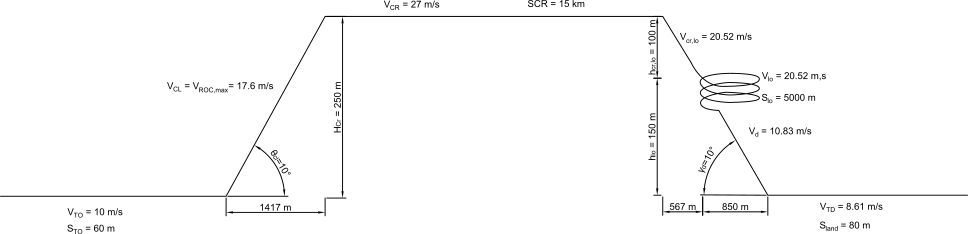
\includegraphics[width=\linewidth]{Mission Profile.png}
\end{figure}

\section{Data collection}
Here is the list of similar airplanes:-


\subsection{WingtraOne}

\begin{figure}[h]
    \begin{minipage}[b]{.45\linewidth}
        \centering
        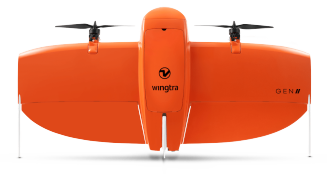
\includegraphics[width=0.7\linewidth]{Aircraft pics/WingtraOne.png}
        
    \end{minipage}\hfill
    \begin{minipage}[b]{0.45\linewidth}
        \begin{itemize}
            \item [-] Takeoff weight: 4.2 kg
            \item [-] Powerplant: Electric motors
            \item [-] Max speed: 150 km/h 
            \item [-] Cruising speed: 85 kph 
            \item [-] Endurance: 55 minutes
        \end{itemize}
    \end{minipage}
\end{figure}

\vspace{\fill}

\clearpage

\subsection{Phoenix Ace Core}
\begin{figure}[h]
    \begin{minipage}[b]{.45\linewidth}
        \centering
        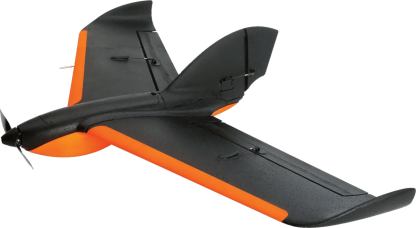
\includegraphics[width=0.7\linewidth]{Aircraft pics/Pheonix Ace core.png}       
    \end{minipage}\hfill
    \begin{minipage}[b]{0.45\linewidth}
        \begin{itemize}
            \item [-] Takeoff weight: 6.2 kg
            \item [-] Powerplant: Electric motors
            \item [-] Max speed: 95 km/h 
            \item [-] Cruising speed: 90 kph 
            \item [-] Endurance: 75 minutes
        \end{itemize}
    \end{minipage}
\end{figure}

\vspace{\fill}

\subsection{Trimble UX5 HP}
\begin{figure}[h]
    \begin{minipage}[b]{.45\linewidth}
        \centering
        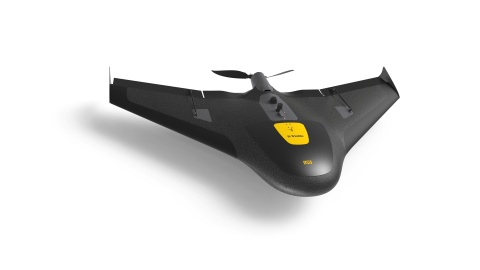
\includegraphics[width=0.7\linewidth]{Aircraft pics/Trimble Ux5 hp.png}
        
    \end{minipage}\hfill
    \begin{minipage}[b]{0.45\linewidth}
        \begin{itemize}
            \item [-] Takeoff weight: 2 kg
            \item [-] Powerplant: Electric motors
            \item [-] Max speed: 90 km/h 
            \item [-] Cruising speed: 72 kph 
            \item [-] Endurance: 50 minutes
        \end{itemize}
    \end{minipage}
\end{figure}

\vspace{\fill}

\subsection{Sensefly eBee Classic}
\begin{figure}[h]
    \begin{minipage}[b]{.45\linewidth}
        \centering
        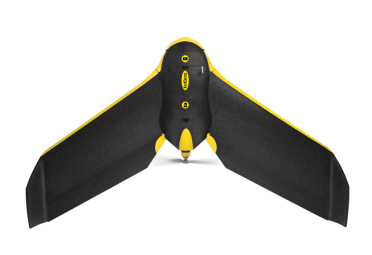
\includegraphics[width=0.7\linewidth]{Aircraft pics/Sensefly ebee classic.png}
    \end{minipage}\hfill
    \begin{minipage}[b]{0.45\linewidth}
        \begin{itemize}
            \item [-] Takeoff weight: 0.7 kg
            \item [-] Powerplant: Electric motors
            \item [-] Max speed: 90 km/h 
            \item [-] Cruising speed: 45-55 km/h 
            \item [-] Endurance: 45 minutes
        \end{itemize}
    \end{minipage}
\end{figure}

\vspace{\fill}
\clearpage

\subsection{Zala 421-08}
\begin{figure}[h]
    \begin{minipage}[b]{.45\linewidth}
        \centering
        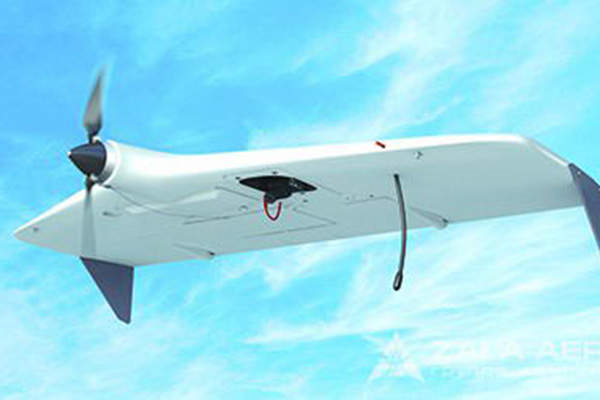
\includegraphics[width=0.7\linewidth]{Aircraft pics/zala 421-08.png}
    \end{minipage}\hfill
    \begin{minipage}[b]{0.45\linewidth}
        \begin{itemize}
            \item [-] Takeoff weight: 5.3 kg
            \item [-] Powerplant: Gasoline
            \item [-] Max speed: 130 km/h 
            \item [-] Cruising speed: 40-50 km/h 
            \item [-] Endurance: 5 hours
        \end{itemize}
    \end{minipage}
\end{figure}

\vspace{\fill}


\subsection{IAI Bird Eye 650}
\begin{figure}[h]
    \begin{minipage}[b]{.45\linewidth}
        \centering
        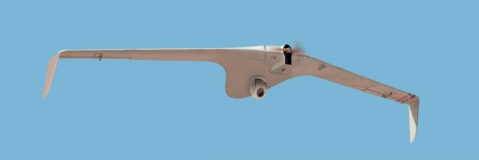
\includegraphics[width=0.7\linewidth]{Aircraft pics/IAI Bird Eye 650.png}
    \end{minipage}\hfill
    \begin{minipage}[b]{0.45\linewidth}
        \begin{itemize}
            \item [-] Takeoff weight: 6.5 kg
            \item [-] Powerplant: Gasoline Engine
            \item [-] Max speed: 120 km/h 
            \item [-] Cruising speed: 50-55 km/h 
            \item [-] Endurance: 4 hours
        \end{itemize}
    \end{minipage}
\end{figure}

\vspace{\fill}

\subsection{Albatross fixed wing UAV}
\begin{figure}[h]
    \begin{minipage}[b]{.45\linewidth}
        \centering
        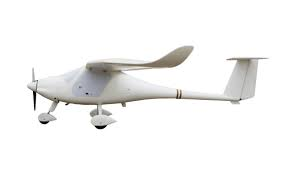
\includegraphics[width=0.7\linewidth]{Aircraft pics/Albatross Fixed wing UAV.png}
    \end{minipage}\hfill
    \begin{minipage}[b]{0.45\linewidth}
        \begin{itemize}
            \item [-] Range : 100 km
            \item [-] Takeoff weight: 10 kg
            \item [-] Powerplant: Battery power single propeller
            \item [-] Max speed: 140 km/h 
            \item [-] Cruising speed: 64 km/h 
            \item [-] Endurance: 5 hours
        \end{itemize}
    \end{minipage}
\end{figure}

\vspace{\fill}
\clearpage

\subsection{Skyle 2 electric UAV}
\begin{figure}[h]
    \begin{minipage}[b]{.45\linewidth}
        \centering
        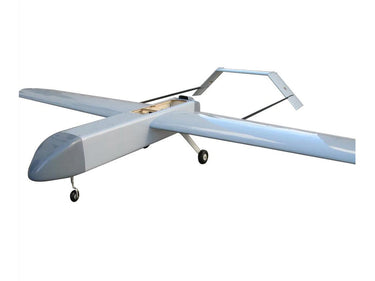
\includegraphics[width=0.7\linewidth]{Aircraft pics/Skyeye.png}
    \end{minipage}\hfill
    \begin{minipage}[b]{0.45\linewidth}
        \begin{itemize}
            \item [-] Takeoff weight: 12 kg
            \item [-] Powerplant: Battery powered single propeller
            \item [-] Max speed: 100 km/h 
            \item [-] Payload weight : 3 kg
%            \item [-] Cruising speed: 50-55 km/h 
            \item [-] Endurance: 1 hours
        \end{itemize}
    \end{minipage}
\end{figure}

\vspace{\fill}


\subsection{Skyeye 50CC Teaching Plane}
\begin{figure}[h]
    \begin{minipage}[b]{.45\linewidth}
        \centering
        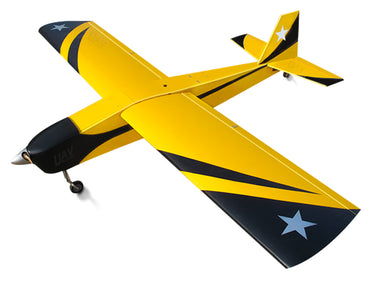
\includegraphics[width=0.7\linewidth]{Aircraft pics/. SKYEYE 50CC.png}
    \end{minipage}\hfill
    \begin{minipage}[b]{0.45\linewidth}
        \begin{itemize}
            \item [-] Takeoff weight: 15 kg
            \item [-] Powerplant: 50CC Gasoline Engine
%            \item [-] Max speed: 120 km/h 
            \item [-] Cruising speed: 100 km/h 
            \item [-] Payload Weight : 6 kg
%            \item [-] Endurance: 4 hours
        \end{itemize}
    \end{minipage}
\end{figure}

\vspace{\fill}

\subsection{Makefly FIghter}
\begin{figure}[h]
    \begin{minipage}[b]{.45\linewidth}
        \centering
        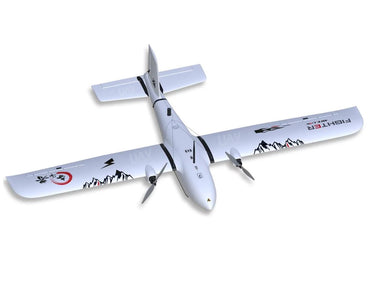
\includegraphics[width=0.7\linewidth]{Aircraft pics/MAKEFLYEASY FIGHTER.png}
    \end{minipage}\hfill
    \begin{minipage}[b]{0.45\linewidth}
        \begin{itemize}
            \item [-] Takeoff weight: 11.5 kg
            \item [-] Powerplant: Battery powered two propeller
            \item [-] Cruising speed : 72 km/h 
            \item [-] Range : 250 km 
            \item [-] Payload weight : 1.5 kg
        \end{itemize}
    \end{minipage}
\end{figure}

\vspace{\fill}
\clearpage

\subsection{Skyeye Swallow fixed wing UAV}
\begin{figure}[h]
    \begin{minipage}[b]{.45\linewidth}
        \centering
        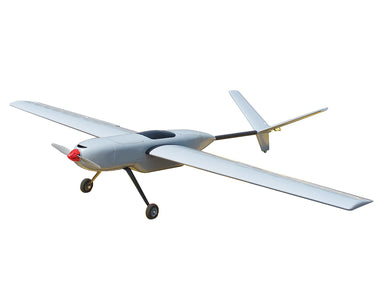
\includegraphics[width=0.7\linewidth]{Aircraft pics/SKYEYE SWALLOW.png}
    \end{minipage}\hfill
    \begin{minipage}[b]{0.45\linewidth}
        \begin{itemize}
            \item [-] Takeoff weight: 9 kg
            \item [-] Powerplant: Battery powered Single propeller
            \item [-] Payload weight : 4 kg
%            \item [-] Cruising speed: 50-55 km/h 
            \item [-] Endurance: 2 hours
        \end{itemize}
    \end{minipage}
\end{figure}

\vspace{\fill}


\subsection{UAVOS Sitaria E^{\ref{MFD}}}
\begin{figure}[h]
    \begin{minipage}[b]{.45\linewidth}
        \centering
        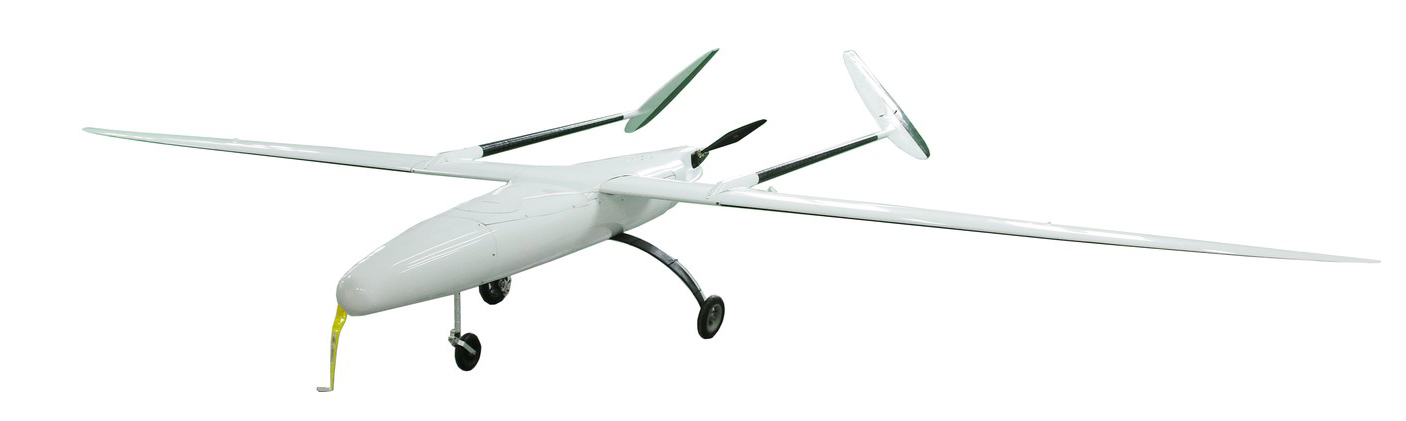
\includegraphics[width=0.7\linewidth]{Aircraft pics/UAVOS SITARIA E.png}
    \end{minipage}\hfill
    \begin{minipage}[b]{0.45\linewidth}
        \begin{itemize}
            \item [-] Range : 240 km
            \item [-] Takeoff weight: 18 kg
            \item [-] Powerplant: Battery powered 2 propellers
            \item [-] Payload weight : 8 kg
            \item [-] Cruising speed: 80 km/h 
            \item [-] Endurance: 3 hours
        \end{itemize}
    \end{minipage}
\end{figure}



\vspace{\fill}

\section{References}
\begin{enumerate}
    \item \label{MFD} \href{https://www.uavmodel.com/collections/fixed-wing/products/mfd-crosswind-nimbus-pro-v2-binary-1900mm-uav-fixed-wing}{MFD}
\end{enumerate}

\end{document}
